% Graphic for TeX using PGF
% Title: /tmp/Diagram1.dia
% Creator: Dia v0.95
% CreationDate: Sun Oct 25 13:49:40 2009
% For: kapranov
% \usepackage{tikz}
% The following commands are not supported in PSTricks at present
% We define them conditionally, so when they are implemented,
% this pgf file will use them.
\ifx\du\undefined
  \newlength{\du}
\fi
\setlength{\du}{15\unitlength}
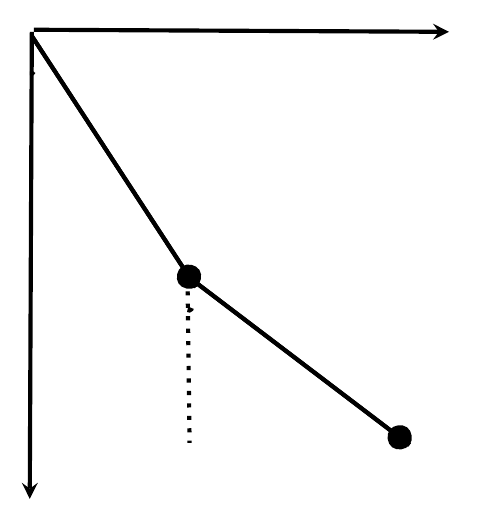
\begin{tikzpicture}
\pgftransformxscale{1.000000}
\pgftransformyscale{-1.000000}
\definecolor{dialinecolor}{rgb}{0.000000, 0.000000, 0.000000}
\pgfsetstrokecolor{dialinecolor}
\definecolor{dialinecolor}{rgb}{1.000000, 1.000000, 1.000000}
\pgfsetfillcolor{dialinecolor}
\pgfsetlinewidth{0.100000\du}
\pgfsetdash{}{0pt}
\pgfsetdash{}{0pt}
\pgfsetbuttcap
{
\definecolor{dialinecolor}{rgb}{0.000000, 0.000000, 0.000000}
\pgfsetfillcolor{dialinecolor}
% was here!!!
\pgfsetarrowsend{stealth}
\definecolor{dialinecolor}{rgb}{0.000000, 0.000000, 0.000000}
\pgfsetstrokecolor{dialinecolor}
\draw (5.050000\du,2.100000\du)--(15.050000\du,2.150000\du);
}
\pgfsetlinewidth{0.100000\du}
\pgfsetdash{}{0pt}
\pgfsetdash{}{0pt}
\pgfsetbuttcap
{
\definecolor{dialinecolor}{rgb}{0.000000, 0.000000, 0.000000}
\pgfsetfillcolor{dialinecolor}
% was here!!!
\pgfsetarrowsend{stealth}
\definecolor{dialinecolor}{rgb}{0.000000, 0.000000, 0.000000}
\pgfsetstrokecolor{dialinecolor}
\draw (5.000000\du,2.150000\du)--(4.950000\du,13.400000\du);
}
\pgfsetlinewidth{0.100000\du}
\pgfsetdash{}{0pt}
\pgfsetdash{}{0pt}
\pgfsetbuttcap
{
\definecolor{dialinecolor}{rgb}{0.000000, 0.000000, 0.000000}
\pgfsetfillcolor{dialinecolor}
% was here!!!
\definecolor{dialinecolor}{rgb}{0.000000, 0.000000, 0.000000}
\pgfsetstrokecolor{dialinecolor}
\draw (5.000000\du,2.250000\du)--(8.950000\du,8.300000\du);
}
\definecolor{dialinecolor}{rgb}{0.000000, 0.000000, 0.000000}
\pgfsetstrokecolor{dialinecolor}
\draw (5.000000\du,2.250000\du)--(8.950000\du,8.300000\du);
\pgfsetlinewidth{0.100000\du}
\pgfsetdash{}{0pt}
\pgfsetmiterjoin
\pgfsetbuttcap
\definecolor{dialinecolor}{rgb}{0.000000, 0.000000, 0.000000}
\pgfsetfillcolor{dialinecolor}
\pgfpathmoveto{\pgfpoint{8.950000\du}{8.300000\du}}
\pgfpathcurveto{\pgfpoint{8.824400\du}{8.382003\du}}{\pgfpoint{8.616796\du}{8.338407\du}}{\pgfpoint{8.534792\du}{8.212806\du}}
\pgfpathcurveto{\pgfpoint{8.452789\du}{8.087206\du}}{\pgfpoint{8.496386\du}{7.879602\du}}{\pgfpoint{8.621986\du}{7.797599\du}}
\pgfpathcurveto{\pgfpoint{8.747586\du}{7.715595\du}}{\pgfpoint{8.955190\du}{7.759192\du}}{\pgfpoint{9.037194\du}{7.884792\du}}
\pgfpathcurveto{\pgfpoint{9.119197\du}{8.010393\du}}{\pgfpoint{9.075600\du}{8.217997\du}}{\pgfpoint{8.950000\du}{8.300000\du}}
\pgfusepath{fill}
\pgfsetlinewidth{0.100000\du}
\pgfsetdash{}{0pt}
\pgfsetdash{}{0pt}
\pgfsetbuttcap
{
\definecolor{dialinecolor}{rgb}{0.000000, 0.000000, 0.000000}
\pgfsetfillcolor{dialinecolor}
% was here!!!
\definecolor{dialinecolor}{rgb}{0.000000, 0.000000, 0.000000}
\pgfsetstrokecolor{dialinecolor}
\draw (8.900000\du,8.150000\du)--(14.100000\du,12.100000\du);
}
\definecolor{dialinecolor}{rgb}{0.000000, 0.000000, 0.000000}
\pgfsetstrokecolor{dialinecolor}
\draw (8.900000\du,8.150000\du)--(14.100000\du,12.100000\du);
\pgfsetlinewidth{0.100000\du}
\pgfsetdash{}{0pt}
\pgfsetmiterjoin
\pgfsetbuttcap
\definecolor{dialinecolor}{rgb}{0.000000, 0.000000, 0.000000}
\pgfsetfillcolor{dialinecolor}
\pgfpathmoveto{\pgfpoint{14.100000\du}{12.100000\du}}
\pgfpathcurveto{\pgfpoint{14.009267\du}{12.219446\du}}{\pgfpoint{13.799087\du}{12.248160\du}}{\pgfpoint{13.679640\du}{12.157426\du}}
\pgfpathcurveto{\pgfpoint{13.560194\du}{12.066693\du}}{\pgfpoint{13.531481\du}{11.856513\du}}{\pgfpoint{13.622214\du}{11.737067\du}}
\pgfpathcurveto{\pgfpoint{13.712948\du}{11.617620\du}}{\pgfpoint{13.923127\du}{11.588907\du}}{\pgfpoint{14.042574\du}{11.679640\du}}
\pgfpathcurveto{\pgfpoint{14.162020\du}{11.770374\du}}{\pgfpoint{14.190733\du}{11.980554\du}}{\pgfpoint{14.100000\du}{12.100000\du}}
\pgfusepath{fill}
\pgfsetlinewidth{0.100000\du}
\pgfsetdash{{\pgflinewidth}{0.200000\du}}{0cm}
\pgfsetdash{{\pgflinewidth}{0.200000\du}}{0cm}
\pgfsetbuttcap
{
\definecolor{dialinecolor}{rgb}{0.000000, 0.000000, 0.000000}
\pgfsetfillcolor{dialinecolor}
% was here!!!
\definecolor{dialinecolor}{rgb}{0.000000, 0.000000, 0.000000}
\pgfsetstrokecolor{dialinecolor}
\draw (8.750000\du,8.100000\du)--(8.800000\du,12.050000\du);
}
\pgfsetlinewidth{0.100000\du}
\pgfsetdash{}{0pt}
\pgfsetdash{}{0pt}
\pgfsetbuttcap
{
\definecolor{dialinecolor}{rgb}{0.000000, 0.000000, 0.000000}
\pgfsetfillcolor{dialinecolor}
% was here!!!
\definecolor{dialinecolor}{rgb}{0.000000, 0.000000, 0.000000}
\pgfsetstrokecolor{dialinecolor}
\pgfpathmoveto{\pgfpoint{4.949979\du}{3.149988\du}}
\pgfpatharc{120}{17}{0.343853\du/0.343853\du}
\pgfusepath{stroke}
}
\pgfsetlinewidth{0.100000\du}
\pgfsetdash{}{0pt}
\pgfsetdash{}{0pt}
\pgfsetbuttcap
{
\definecolor{dialinecolor}{rgb}{0.000000, 0.000000, 0.000000}
\pgfsetfillcolor{dialinecolor}
% was here!!!
\definecolor{dialinecolor}{rgb}{0.000000, 0.000000, 0.000000}
\pgfsetstrokecolor{dialinecolor}
\pgfpathmoveto{\pgfpoint{8.749975\du}{8.849982\du}}
\pgfpatharc{126}{9}{0.447834\du/0.447834\du}
\pgfusepath{stroke}
}
\end{tikzpicture}
